\documentclass[10pt]{beamer}
\usepackage{amsmath, graphicx, textcomp,multirow,subfigure, soul, color}

\usetheme{Rochester}
%\usetheme{PaloAlto}
\setbeamertemplate{footline}{\insertframenumber/\inserttotalframenumber}

\newcommand{\true}{{\mbox{\hspace*{0cm}\tiny{\sf true}} }}
\newcommand{\means}{{\mbox{\hspace*{0cm}\tiny{\sf means}} }}
\newcommand{\logit}{\ensuremath{\mbox{logit}}}

\title{Learning with an Unreliable Teacher}
\author{Elizabeth M. Sweeney}
\institute{Department of Biostatistics  \\ Johns Hopkins Bloomberg School of Public Health}
\date{December 11, 2014}

\begin{document}

\frame{\titlepage}
 
\frame{
	\frametitle{ Learning with an Unreliable Teacher}

Lugosi, Gabor. ``Learning with an unreliable teacher." Pattern Recognition 25.1 (1992): 79-87.

\bigskip 

Devroye, Luc, Laszlo Gyorfi, and Gabor Lugosi. A probabilistic theory of pattern recognition. Springer Verlag, 1996.
}


 
%% \frame{
%%	\frametitle{ Abstract}

%%`` In nonparametric pattern recognition problems one has to ``learn" a good decision rule from a long training sequence, that is, independent pairs of observations and corresponding labels .  In many practical situations there may be errors among the labels of the training sequence, that is, ``the teacher may sometimes lie".  In this paper we investigate the behavior of two widely used methods in this situation under very general conditions.  One of these methods is based on the maximization of the estimated a posterior probabilities, the other is nearest neighbor classification. "
%%}




\frame{ 
\frametitle{The Classification Task}

\begin{enumerate} 
\item We have random variables $(X,Y)$ such that  $X \in \mathbb{R}^d$ and $Y \in \{0, 1 \}$. 
\item Let $g: \mathbb{R}^d \rightarrow \{0, 1\}$ 
\item The error probability is $P_g \left( X, Y \right) = \mathbb{P}  \{ g (X) \neq Y \}$
\item The classification task is to find $g$ that minimizes $P_g \left( X, Y \right)$
\end{enumerate} 

}

\frame{ 
\frametitle{The Classification Task}

\begin{enumerate} 
\item In practice we have a training sequence $\xi_n = \left( (X_1, Y_1), (X_2, Y_2), ... (X_n, Y_n)  \right)$  where $\left(X_k, Y_k \right)$ are iid from $\left(X, Y \right) $
\item We then estimate $Y$ from $g_n \left(X, \xi_n \right)$, minimizing $  \mathbb{P}  \{ g_n (X, \xi_n) \neq Y \}$
\end{enumerate} 

}


\frame{
	\frametitle{ Learning with an Unreliable Teacher}
Classification Methods 	
\begin{enumerate} 
\item Bayes decision rule
\item One nearest neighbor  
\end{enumerate}

\bigskip 

Mislabeling Mechanism 	
\begin{enumerate} 
\item Discrete Memoryless Channel 
\item Misprints in the Training Sequence 
\item Consequently Lying Teacher   
\end{enumerate}



}

\frame{
	\frametitle{Some Context}

\begin{figure}
\includegraphics[width=.9\linewidth]{Example1.pdf}
\end{figure} 




}



\frame{ 
\frametitle{ The Bayes Decision Rule }

We wish to find that $g$ such that the error probability $P_g \left( X, Y \right) =  \mathbb{P}  \{ g (X) \neq Y \} $ is minimized.  Let $p_i \left( x \right) =  \mathbb{P} \{ Y = i | X = x \} $, $i \in \{0, 1 \}$.  The optimal solution is the Bayes decision rule:

\bigskip 

\begin{equation}
g^{*} \left(x \right) = \text{argmax }_{0 \leq i \leq 1}  p_i \left( x \right)  \nonumber 
\end{equation} 

\bigskip 

Where optimality is defined as $ \mathbb{P}  \{ g^{*} (X) \neq Y \} \leq  \mathbb{P}  \{ g (X) \neq Y \}$ for all $g$.  We will denote $ \mathbb{P}  \{ g^{*} (X) \neq Y \} $ as $P^{B} \left(X, Y \right)$, which is called the Bayes risk. 
}


\frame{ 
\frametitle{ The Bayes Decision Rule  }

We will often not know $p_i \left( x \right)$, and so we will estimate the with $q_i \left(x, \xi \right)$ with training data $\xi$ and will use the corresponding decision rule 

\begin{equation} 
g \left( x, \xi \right) = \text{argmax}_{i}  q_i \left( x, \xi \right)  \nonumber 
\end{equation} 

}

\frame{ 
\frametitle{ Lemma 1.1  }

The error of probability of the decision $g$ is close to the Bayes risk if the $q_i$ are good $L_1$ approximations of the true posterior probabilities 

\begin{equation}
 \mathbb{P}   \left\{ g(X, \xi ) \neq Y  \right\} - P^{B} \left(X, Y \right) \leq E \left( \sum_{i = 1} ^{1} |p_i \left(X \right) - q_i \left(X, \xi \right) | \right) \nonumber
 \end{equation} 

}

%% \frame{ 
%%\frametitle{ Lemma 1.2  }

%%A stronger version of Lemma 1.2 

%%\begin{align} 
%% \mathbb{P}   \left\{ g(X, \xi ) \neq Y  \right\} - P^{B} \left(X, Y \right)  &\leq E \left( \sum_{i = 0}^{1} | p_i \left(X \right) - q_i \left(X, \xi \right) | \big | g \left(X, \xi \right) \neq g^{*} \left( X \right) \right) \nonumber \\
%% & \times  \mathbb{P}  \{ g \left(X, \xi \right) \neq g^{*} \left(X \right) \} 
%%\end{align}


%%}


\frame{ 
\frametitle{ Lemma 1.3 }


\bigskip 

Let $q_0 \left(x \right)$ and $q_1 \left( x \right)$ be real valued measurable functions defined on $\mathbb{R}^d$.  Let the decision function $g$ be the following: 

\begin{equation} 
g \left(x \right) = \text{argmax}_i q_i \left(x \right)  \nonumber 
\end{equation} 

If this maximum is unique almost everywhere then for any sequence of measurable functions $\bar{q}_i ^{(n )}  \left( x, s \right)$ $\left( i = 0, 1; n = 1,2, ... \right)$, for which 

\begin{equation}
\lim_{n \rightarrow \infty} E \left( \sum_{i = 0} ^{1} | q_i \left(X \right) - \bar{q}_i ^{(n )} \left(X, \xi \right)   | \right) = 0 \nonumber 
\end{equation}
}


\frame{ 
\frametitle{ Lemma 1.3 }

then 

\begin{equation} 
\lim | P_g \left(X, Y \right) - P_{\bar{g} ^{(n)} } \left(X, Y \right) | = 0 \nonumber 
\end{equation} 

where 

\begin{equation} 
\bar{g} ^{(n)} \left(x, s \right) = \text{argmax}_i \bar{q}_i ^{(n )}  \left(x, s \right) \nonumber 
\end{equation} 

\bigskip 

``Every decision based on maximization of measurable functions can be arbitrarily approximated by approximating the function in the $L_1$ sense "
}




\frame{ 
\frametitle{ Proof of Lemma 1.3 }

\textbf{Proof:}  We first note that 

\begin{align} 
P_g \left(X, Y \right) &=   \mathbb{P}  \left( g(X) \neq Y \right) \nonumber \\
 &=  1 -  \mathbb{P}  \left( g(X) = Y \right) \nonumber \\
  &=  1 -  E \left[  I_{ \left( g(X) = Y \right) } \right]  \nonumber 
\end{align} 


The difference between the error of probabilities is then 

\begin{align} 
 | P_g \left(X, Y \right) - P_{\bar{g} ^{(n)} } \left(X, Y \right) |  &=  \left| E \left[  I_{ \left( \bar{g}^{(n)}  \left(X, \xi \right)  = Y \right) } \right]  - E \left[  I_{ \left( g(X) = Y \right) } \right]  \right| \nonumber \\
 &= \left| E \left[  I_{ \left( \bar{g}^{(n)}  \left(X, \xi \right)  = Y \right) }  -  I_{ \left( g(X) = Y \right) } \right] \right|   \nonumber
\end{align} 
}

\frame{ 
\frametitle{ Proof of Lemma 1.3 }

Then we have that 

\begin{align} 
 \left| E \left[  I_{ \left( \bar{g}^{(n)}  \left(X, \xi \right)  = Y \right) }  -  I_{ \left( g(X) = Y \right) } \right] \right|   & \leq  E   \left[  \left|  I_{ \left( \bar{g}^{(n)}  \left(X, \xi \right)  = Y \right) }  -  I_{ \left( g(X) = Y \right) }   \right|   \right]  \nonumber \\
  & =   E   \left[   I_{ \left( \bar{g}^{(n)}  \left(X, \xi \right)  \neq g \left( X \right)  \right) }   \right]  \nonumber \\
& = \mathbb{P} \{ g \left(X \right) \neq \bar{g}^{(n)} \left(X, \xi \right) \} \nonumber 
 \end{align} 

 
}



\frame{ 
\frametitle{ Proof of Lemma 1.3 }

Therefore 

\begin{align} 
 | P_g \left(X, Y \right) - P_{\bar{g} ^{(n)} } \left(X, Y \right) |  & \leq  \mathbb{P} \{ g \left(X \right) \neq \bar{g}^{(n)} \left(X, \xi \right) \}  \nonumber \\
&=  \mathbb{P}   \{ g \left(X \right) = 1, \bar{g}^{(n)} \left(X, \xi \right) = 0 \} \nonumber \\
& + \mathbb{P}   \{ g \left(X \right) = 0, \bar{g}^{(n)} \left(X, \xi \right) = 1 \}  \nonumber 
\end{align} 
 
}



\frame{ 
\frametitle{ Proof of Lemma 1.3 }

By symmetry, we need only show that as $n \rightarrow \infty$ 

\begin{equation} 
\mathbb{P}  \{ g \left(X \right) = 1, \bar{g}^{(n)} \left(X, \xi \right) = 0  \} \rightarrow 0 \nonumber 
\end{equation} 

For all $ \delta > 0$ we have that 

\begin{align} 
\mathbb{P}  \{ g \left(X \right) = 1, \bar{g}^{(n)} \left(X, \xi \right) = 0  \}  &= \mathbb{P} \{ q_1 \left(X \right) \geq q_0 \left(X \right), \bar{q}_1^{n} \left(X, \xi \right) \leq \bar{q}_0^{n} \left(X, \xi \right) \} \nonumber \\
& \leq  \mathbb{P}  \{ | q_1 \left(X \right) - q_0 \left(X \right) | < \delta \}   \nonumber \\
& +  \mathbb{P} \left\{ \sum_{i = 0}^{1} |q_i \left(X \right) - \bar{q}_i^{(n)} \left(X, \xi \right) | \geq \delta \right\} \nonumber
\end{align} 



}


\frame{ 
\frametitle{ Proof of Lemma 1.3 }

By symmetry, we need only show that as $n \rightarrow \infty$ 

\begin{equation} 
\mathbb{P}  \{ g \left(X \right) = 1, \bar{g}^{(n)} \left(X, \xi \right) = 0  \} \rightarrow 0 \nonumber 
\end{equation} 

For all $ \delta > 0$ we have that 

\begin{align} 
\mathbb{P}  \{ g \left(X \right) = 1, \bar{g}^{(n)} \left(X, \xi \right) = 0  \}  &= \mathbb{P} \{ q_1 \left(X \right) \geq q_0 \left(X \right), \bar{q}_1^{n} \left(X, \xi \right) \leq \bar{q}_0^{n} \left(X, \xi \right) \} \nonumber \\
&  \color {red} {  \leq  \mathbb{P}  \{ | q_1 \left(X \right) - q_0 \left(X \right) | < \delta \}  }   \nonumber \\
& \color {red} { +  \mathbb{P} \left\{ \sum_{i = 0}^{1} |q_i \left(X \right) - \bar{q}_i^{(n)} \left(X, \xi \right) | \geq \delta \right\}  }\nonumber
\end{align} 



}



\frame{ 
\frametitle{ Learning with an Unreliable Teacher  }

\begin{figure}
\includegraphics[width=.9\linewidth]{Email.png}
\end{figure} 



}



\frame{ 
\frametitle{ Proof of Lemma 1.3 }

We now show that for any $\epsilon > 0 $, we can chose $\delta$ and $N$ such that if $n > N$ we have 

\begin{equation} 
 \mathbb{P}  \{ | q_1 \left(X \right) - q_0 \left(X \right) | < \delta \}  +  \mathbb{P} \left\{ \sum_{i = 0}^{1} |q_i \left(X \right) - \bar{q}_i^{(n)} \left(X, \xi \right) | \geq \delta \right\} < \epsilon \nonumber 
\end{equation} 
}


\frame{ 
\frametitle{ Proof of Lemma 1.3 }

We have that the maximum of $q_i \left( x \right)$ is unique almost everywhere, therefore 

\begin{equation} 
|q_1 \left( X \right) - q_0 \left(X \right) | > 0 \nonumber 
\end{equation} 

with probability 1 and so a $\delta$ can be selected such that 

\begin{equation} 
 \mathbb{P}  \{ | q_1 \left(X \right) - q_0 \left(X \right) | < \delta \}  < \frac{ \epsilon}{2} \nonumber 
\end{equation} 
}



\frame{ 
\frametitle{ Proof of Lemma 1.3 }

By the $L_1$ convergence of the function $\bar {q}_i ^{(n)} \left(x, s \right)$ 


\begin{equation} 
\lim_{n \rightarrow \infty} \mathbb{P} \left\{ \sum_{i = 0}^{1} |q_i \left(X \right) - \bar{q}_i^{(n)} \left(X, \xi \right) | \geq \delta \right\} =  0  \nonumber 
\end{equation} 

therefore, there exists an $N$ such that for every $n > N$ we have 

\begin{equation} 
 \mathbb{P} \left\{ \sum_{i = 0}^{1} |q_i \left(X \right) - \bar{q}_i^{(n)} \left(X, \xi \right) | \geq \delta \right\}  < \frac{ \epsilon}{2} \nonumber 
\end{equation} 

\begin{flushright}
$\square$ 
\end{flushright}
}


\frame{ 
\frametitle{Labeling Errors in the Training Set }

\begin{enumerate} 
\item We deal with the case where instead of knowing $Y_k$ we have the labels $Z_k \in \{0, 1\} $ which are erroneous labels 
\item Let $\left(X_k, Y_k, Z_k \right)$  be iid from  $\left(X,Y, Z\right)$    
\item We now wish to estimate $Y$ given the data $X$ from the training set $\eta_n =  \left( (X_1, Z_1), (X_2, Z_2), ... (X_n, Z_n)  \right)  $                                                           
\end{enumerate} 

}






\frame{ 
\frametitle{ Bayes Decision Rule with Mislabeled Training Data }

Let  $q_i (x) =  \mathbb{P} \{ Z = i | X = x \}$.  We assume that we have an $L_1$ consistent estimator of $q_i (x)$ and we will denote this estimator by $q_{in} \left(x \right) = q_{in} \left(x, \eta_n \right)$.  By $L_1$ consistency we will mean 

\begin{equation} 
\lim_{n \rightarrow \infty} E \left( \sum_{i = 0}^{1} | q_i \left(X \right) - q_{in} \left(X \right) | \right) = 0 \nonumber 
\end{equation} 

and the corresponding decision rule will be 

\begin{equation} 
g_n \left(x \right) = \text{argmax}_i q_{in} \left(x \right) \nonumber 
\end{equation} 

which is an approximation of $g(x) =  \text{argmax}_i q_{i} \left(x \right)$


}


%% \frame{ 
%% \frametitle{ Theorem 2.1 }

%% If the decision $g$ is unique almost everywhere, then 

%%\begin{equation} 
%%\lim \sup_{n \rightarrow \infty} P_{g_n} \left(X, Y \right) - P^{B} \left(X, Y \right) \leq 2  \mathbb{P} \{ Z \neq Y \} \nonumber 
%%\end{equation} 


%%}



\frame{ 
\frametitle{ Discrete Memoryless Channel }

Here we assume that the true labels $Y_k$ are transmitted over a binary memoryless channel to get the training labels $Z_k$.  


\begin{align} 
a_{ji} & =  \mathbb{P} \{ Z = i | Y = j, X = x \}  \nonumber \\
& =  \mathbb{P} \{ Z = i | Y = j \} \nonumber  
\end{align}
}

\frame{ 
\frametitle{ Discrete Memoryless Channel }

Let 

\begin{equation} 
A = \left(\begin{array}{cc} a_{00} & a_{01}  \\ a_{10}  &  a_{11} \end{array}\right) =  \left(\begin{array}{cc} 1 - p  & p  \\ q  &  1 - q \end{array}\right) \nonumber 
\end{equation}

\bigskip 

then $\textbf{q} \left(x \right) = \left(\begin{array}{cc}q_0\left(x \right)& q_1 \left(x \right)  \end{array}\right)$ and  $\textbf{p} \left(x \right) = \left(\begin{array}{cc}p_0\left(x \right)& p_1 \left(x \right)  \end{array}\right)$.  Then we have that 

\begin{equation} 
\textbf{q} \left(x \right) = \textbf{p} \left(x \right) A \nonumber 
\end{equation} 


}


\frame{ 
\frametitle{ Known Discrete Memoryless Channel }

We focus on the case where the discrete memoryless channel is known.  Let $\textbf{q}_{n}  \left(x \right) = \left(\begin{array}{cc}q_{0n} \left(x \right)& q_{1n} \left(x \right)  \end{array}\right)$.  Let $\textbf{p}_{n} \left(x \right)$ be the solution to the equation $\textbf{q}_{n} \left(x \right) =  \textbf{p}_{n} \left(x \right) A$.  Then define 

\begin{equation} 
f_n \left( x \right) = \text{argmax}_i p_{in} \left( x \right) \nonumber 
\end{equation} 

}


\frame{ 
\frametitle{ Theorem 2.2 }

As long as $p + q \neq 1$ the decision $f_n$ is asymptotically optimal:  
 
\begin{equation} 
P_{f_n} \left(X, Y \right) - P^{B} \left(X, Y \right) \leq \left| \frac{ 1 + |p - q| }{ 1 - p - q}  \right| E \left( \sum_{i = 0}^{1} |q_i \left(X \right) - q_{in} \left(X \right) | \right) \nonumber 
\end{equation} 
}


\frame{ 
\frametitle{ Proof Theorem 2.2 }

We begin by introducing the following notation 

\begin{align} 
\delta_{in} \left(x \right) &= q_i \left(x\right) - q_{in} \left( x \right) \nonumber \\
\gamma_{in} \left(x \right) &= p_i \left(x\right) - p_{in} \left( x \right) \nonumber
\end{align} 

And let $\Delta_n  = \left(\begin{array}{cc}\delta_{0n} \left(x \right)& \delta_{1n} \left(x \right)  \end{array}\right)$ and $\Gamma_n = \left(\begin{array}{cc}\gamma_{0n} \left(x \right)& \gamma_{1n}  \left(x \right)  \end{array}\right)$.  Then, as   $\textbf{q} \left(x \right) = \textbf{p} \left(x \right) A \nonumber $ and $\textbf{q}_{n} \left(x \right) =  \textbf{p}_{n} \left(x \right) A$, it follows that 

\begin{equation} 
\Delta_n \left(x \right) = \Gamma_n \left(x \right) A  \nonumber 
\end{equation} 

}

\frame{ 
\frametitle{ Proof Theorem 2.2 }

Assuming A is invertible, we have 

\begin{equation} 
\Delta_n \left(x \right) A^{-1} = \Gamma_n \left(x \right) \nonumber 
\end{equation} 

We then take the $L_1$ norm of both sides of the equation 

\begin{equation} 
\sum_{i = 0}^{1} |p_i \left(x \right) - p_{in} \left(x \right) | = \sum_{i=0}^{1} |q_{i}\left( x \right) - q_{in} \left( x \right) | \| A^{-1} \|_1 \nonumber 
\end{equation} 

where 

\begin{equation} 
 \| A^{-1} \|_1 = \left| \frac{ 1 + | p - q | }{ 1 - p - q} \right|  \nonumber 
\end{equation} 



}



\frame{ 
\frametitle{ Proof Theorem 2.2 }

Taking the expectation of both sides gives us 
\begin{equation} 
E  \sum_{i = 0}^{1} |p_i \left(x \right) - p_{in} \left(x \right) | =  \left| \frac{ 1 + | p - q | }{ 1 - p - q} \right|  E \sum_{i=0}^{1} |q_{i}\left( x \right) - q_{in} \left( x \right) |  \nonumber 
\end{equation} 



Applying Lemma 1.1 will give us that 

\begin{equation} 
P_{f_n} \left( X, Y \right) - P^{B} \left(X, Y \right) \leq E \sum_{i = 0}^{1} |p_i \left(x \right) - p_{in} \left(x \right) | \nonumber 
\end{equation} 


and therefore 

\begin{equation} 
P_{f_n} \left(X, Y \right) - P^{B} \left(X, Y \right) \leq \left| \frac{ 1 + |p - q| }{ 1 - p - q}  \right| E \left( \sum_{i = 0}^{1} |q_i \left(X \right) - q_{in} \left(X \right) | \right) \nonumber 
\end{equation} 




}






\frame{ 
\frametitle{ Consequently Lying Teacher  }

For the consequently lying teacher, we have that for $h: \mathbb{R}^d \rightarrow \{0, 1 \}$

\begin{equation} 
Z = h \left(X \right) \nonumber 
\end{equation} 

And in this case 

\begin{equation} 
q_i \left( x \right) =  \mathbb{P}  \{ Z = i | X = x \} =   \mathbb{P} \{ h( X ) = i | X = x \} \nonumber 
\end{equation} 

and so 

\begin{equation} 
q_i \left( x \right)  = \left\{\begin{array}{cc} 1  &  \text{ if h(x) = i}  \\0 &  \text{otherwise} \end{array}\right. \nonumber 
\end{equation} 


therefore $g = h$ and we have that 

\begin{equation} 
 \mathbb{P} \{ g \left(X \right) \neq Y \} =  \mathbb{P} \{ Y \neq Z \} \nonumber 
\end{equation} 

}

\frame{ 
\frametitle{ Conclusion  }

\begin{enumerate} 
\item With the discrete memoryless channel for mislabeling, we can reach Bayes optimal classification error 

\item With the consequently lying teacher, as long as there is mislabeling, we never reach Bayes optimal 
\end{enumerate} 
}



\frame{ 
\frametitle{ Consequently Lying Teacher  }

\begin{figure}
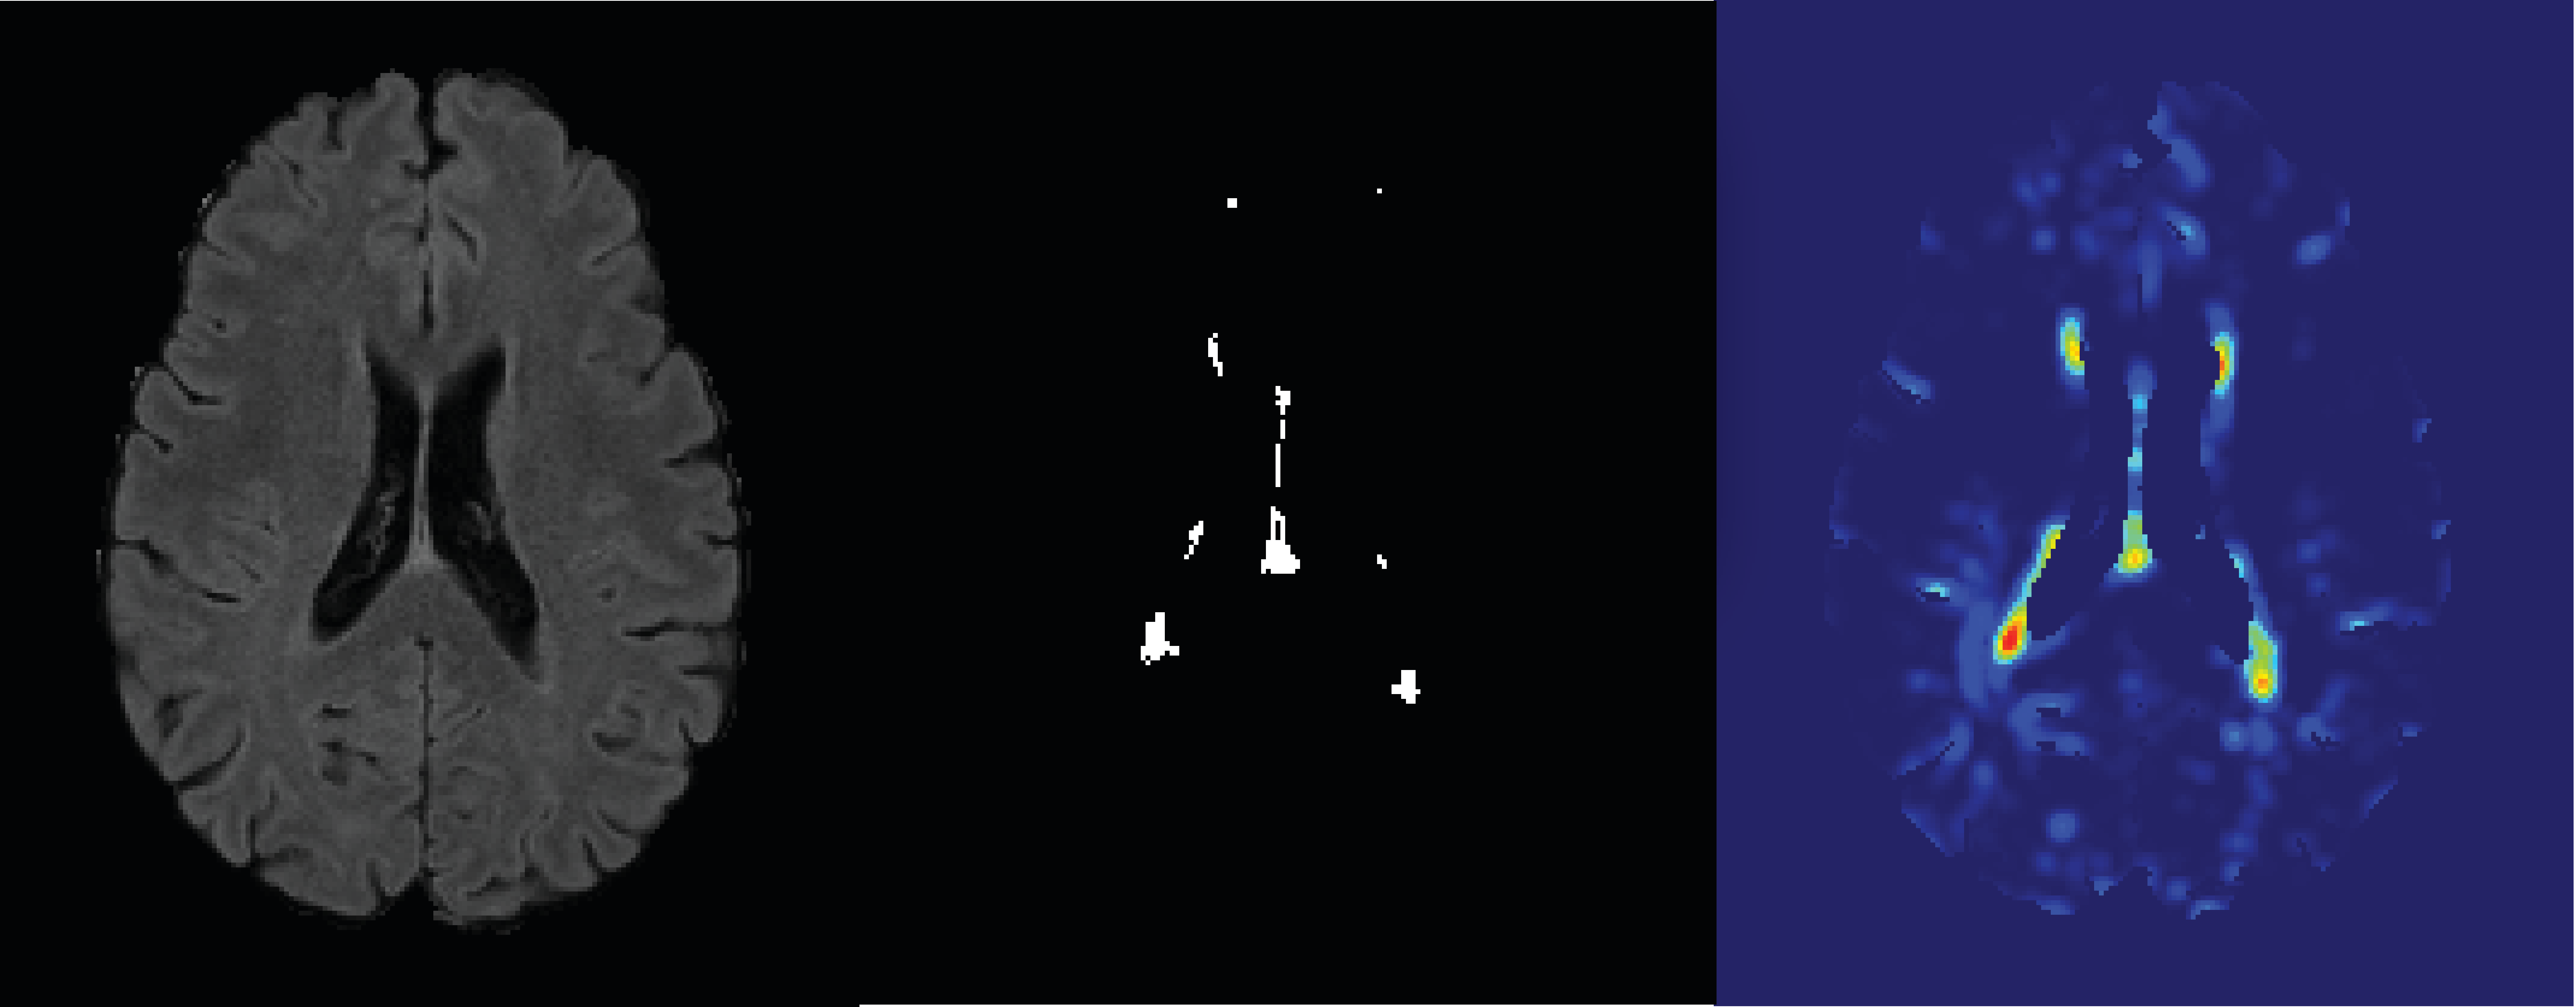
\includegraphics[width=.9\linewidth]{Example2.pdf}
\end{figure} 



}


\frame{ 
\frametitle{ Supplemental Materials }

\begin{enumerate} 
\item Optimality of  the Bayes Decision Rule
\item Misprints in the Training Sequence 
\end{enumerate} 

}










\frame{ 
\frametitle{Optimality of  the Bayes Decision Rule }

\textbf{Proof}: Let $p_i \left( x \right) =  \mathbb{P} \{ Y_i = i | X = x \} $.  For any classifier $g$ we have that 


\begin{align}
\mathbb{P}   \left\{ g (X) \neq Y | X = x \right\} &= 1 - \mathbb{P}   \left\{ g (X) = Y | X = x \right\} \nonumber \\
&= 1 - \mathbb{P}   \left\{ g (X) = 0, Y = 0   | X = x \right\}  \nonumber   \\
&  - \mathbb{P}   \left\{ g (X) = 1, Y = 1   | X = x \right\}  \nonumber \\
& = 1 - I \left( g(x) =0  \right) p_0\left( x \right)  - I \left( g(x) = 1 \right) p_1 \left( x \right)  \nonumber \\
& = 1 - I \left( g(x) =0  \right) p_0\left( x \right)  - I \left( g(x) = 1 \right) ( 1 -  p_0  \left( x \right) ) \nonumber 
\end{align} 


}



\frame{ 
\frametitle{ Optimality of  the Bayes Decision Rule }

Then we have that 


\begin{align}
& \mathbb{P}   \left\{ g (X) \neq Y | X = x \right\}  - \mathbb{P}   \left\{ g^*(X) \neq Y | X = x \right\}   \nonumber \\
&= p_0 \left(x \right) \left(  I \left( g^* (x) =0  \right) -  I \left( g  (x) =0  \right) \right)  +  ( 1 - p_0  \left(x \right) ) \left(  I \left( g^{*} (x) = 1  \right)  \right. \nonumber \\
&  \left. -  I \left( g (x) =1  \right) \right)\nonumber \\
&= p_0 \left(x \right) \left(  I \left( g^{*} (x) =0  \right) -  I \left( g (x) =0  \right) \right)  +  ( 1 - p_0  \left(x \right) ) \left(  \left(  1 -  I \left( g^{*} (x) = 0   \right)  \right)  \right. \nonumber \\
&  \left. -   \left( 1 - I \left( g (x) = 0   \right) \right) \right)\nonumber \\
&= p_0 \left(x \right) \left(  I \left( g^{*} (x) =0  \right) -  I \left( g (x) =0  \right) \right)  +  (  p_0 \left(x \right) - 1) \left(   I \left( g^{*} (x) = 0   \right)  \right. \nonumber \\
&  \left. -   I \left( g (x) = 0   \right) \right)\nonumber \\
&= (2 p_0(x) - 1 ) \left(  I \left( g(x)^{*}  =0  \right) -  I \left( g (x) =0  \right) \right) \nonumber 
\end{align} 



}


\frame{ 
\frametitle{ Optimality of  the Bayes Decision Rule}

And it follows that 

\begin{align}
(2 p_0(x) - 1 ) \left(  I \left( g(x)^{*}  =0  \right) -  I \left( g (x) =0  \right) \right)  \geq 0 \nonumber 
 \end{align} 

as 
\begin{equation}
g^{*} \left(x \right) = \text{argmax }_{0 \leq i \leq 1}  \mathbb{P} \{ Y = i | X = x \}  \nonumber 
\end{equation} 

 therefore when $ I \left( g^{*} (x) =0  \right)   = 1$, $p_0(x) > \frac{1}{2}$ and  when $ I \left( g^{*} (x) =0  \right)   = 0$, $p_0(x) < \frac{1}{2}$.  The proof is completed by integrating both sides with respect to $\mu \left( dx \right)$.   $\square$
}




\frame{ 
\frametitle{ Misprints in the Training Sequence  }

The labels $Z_i$ take an arbitrary value with probability $p$ that is independent from $X_i$ and $Y_i$ 

\begin{equation} 
Z_i = \beta_i Y_i + \left( 1 - \beta_i \right) W_i \nonumber 
\end{equation} 

with $\beta_i \in (0, 1)$, $W_i \in (0, 1)$ and  

\begin{equation}
 \mathbb{P} \left( \beta_i = 0 \right) = p \nonumber 
\end{equation} 

Note that $W_i$ may depend of $X_i$ and $Y_i$ 

}


\frame{ 
\frametitle{ Theorem 2.4  }

When we have misprints in the training sequence the error probability is bounded in the following way for the Bayes decision rule

\begin{equation} 
P_{g} \left(X, Y \right) \leq P^{B} \left(X, Y \right) \frac{1}{1 - 2p} \nonumber 
\end{equation} 


}




\end{document}